\FloatBarrier
\section{Empirical Results}
\label{sec:results}

We evaluate all nine algorithms across 1,000 independent evaluation episodes per checkpoint across 10 random seeds ($10,\!000$ episodes per algorithm per stage, $450,\!000$ total evaluation episodes).

\subsection{Curriculum Scaling \& Benchmark Performance}
\label{sec:benchmark_scaling}

Table~\ref{tab:main_results} and Figure~\ref{fig:curriculum} report the empirical performance across the five curriculum stages. The benchmark demonstrates a clear progression across our iterative method lineage alongside external baselines:

% Benchmark performance across curriculum stages.
\begin{table}[htbp]
\centering
\caption{Empirical benchmark performance across five HEIST curriculum stages ($11\times 11$ to $50\times 50$). Reported as $\text{mean} \pm \text{std}$ evaluated over $N=1,\!000$ episodes across 10 random seeds ($10,\!000$ episodes per cell, $450,\!000$ total evaluation episodes across all nine algorithms under the identical protocol). Partitioned into our iterative development lineage versus external MARL baselines. Bold denotes best performance overall per stage.}
\label{tab:main_results}
\vspace{0.04in}
\footnotesize
\setlength{\tabcolsep}{2.8pt}
\renewcommand{\arraystretch}{1.06}
\begin{tabular}{ll ccccc}
\toprule
 & & \textbf{St. 0 ($11^2$)} & \textbf{St. 1 ($17^2$)} & \textbf{St. 2 ($25^2$)} & \textbf{St. 3 ($35^2$)} & \textbf{St. 4 ($50^2$)} \\
\textbf{Algorithm} & \textbf{Metric} & (0g, 0c) & (1g, 1d) & (2g, 1c, 2d) & (3g, 2c, 3d) & (4g, 3c, 4d) \\
\midrule
\multicolumn{7}{l}{\textit{\textbf{Iterative Method Lineage (Ours)}}} \\
\midrule
\multirow{2}{*}{\textbf{THIEF (Ours, Final)}} & Win Rate & \textbf{100.0\scriptsize$\pm$0.0\%} & \textbf{99.9\scriptsize$\pm$0.1\%} & \textbf{82.2\scriptsize$\pm$1.1\%} & \textbf{39.9\scriptsize$\pm$1.7\%} & \textbf{13.3\scriptsize$\pm$2.4\%} \\
 & Return & \textbf{17.67\scriptsize$\pm$0.04} & \textbf{18.74\scriptsize$\pm$0.04} & \textbf{16.05\scriptsize$\pm$0.36} & \textbf{6.02\scriptsize$\pm$0.43} & \textbf{-1.02\scriptsize$\pm$0.67} \\
\addlinespace[2pt]
\multirow{2}{*}{E-COOP (Iter 3)} & Win Rate & \textbf{100.0\scriptsize$\pm$0.0\%} & 99.8\scriptsize$\pm$0.1\% & 78.0\scriptsize$\pm$1.3\% & 34.5\scriptsize$\pm$2.8\% & 7.6\scriptsize$\pm$1.4\% \\
 & Return & \textbf{17.70\scriptsize$\pm$0.03} & \textbf{18.75\scriptsize$\pm$0.04} & 15.22\scriptsize$\pm$0.32 & 5.30\scriptsize$\pm$0.77 & -1.52\scriptsize$\pm$0.49 \\
\addlinespace[2pt]
\multirow{2}{*}{COOP (Iter 2)} & Win Rate & \textbf{100.0\scriptsize$\pm$0.0\%} & 99.8\scriptsize$\pm$0.1\% & 80.1\scriptsize$\pm$2.9\% & 35.5\scriptsize$\pm$5.3\% & 7.8\scriptsize$\pm$1.7\% \\
 & Return & 17.65\scriptsize$\pm$0.05 & \textbf{18.76\scriptsize$\pm$0.04} & 15.70\scriptsize$\pm$0.69 & 5.52\scriptsize$\pm$1.37 & -1.63\scriptsize$\pm$0.41 \\
\addlinespace[2pt]
\multirow{2}{*}{MARC (Iter 1)} & Win Rate & 99.2\scriptsize$\pm$0.9\% & 99.7\scriptsize$\pm$0.1\% & 81.1\scriptsize$\pm$1.4\% & 31.4\scriptsize$\pm$2.9\% & 6.5\scriptsize$\pm$1.2\% \\
 & Return & 17.32\scriptsize$\pm$0.28 & 18.68\scriptsize$\pm$0.04 & 15.93\scriptsize$\pm$0.33 & 4.47\scriptsize$\pm$0.71 & -2.09\scriptsize$\pm$0.39 \\
\midrule
\multicolumn{7}{l}{\textit{\textbf{External MARL Baselines}}} \\
\midrule
\multirow{2}{*}{ROMA \cite{wang2020roma}} & Win Rate & \textbf{100.0\scriptsize$\pm$0.0\%} & 99.8\scriptsize$\pm$0.1\% & 78.0\scriptsize$\pm$1.8\% & 33.7\scriptsize$\pm$2.1\% & 9.4\scriptsize$\pm$1.2\% \\
 & Return & \textbf{17.71\scriptsize$\pm$0.01} & \textbf{18.74\scriptsize$\pm$0.03} & 15.21\scriptsize$\pm$0.40 & 5.01\scriptsize$\pm$0.60 & \textbf{-1.06\scriptsize$\pm$0.40} \\
\addlinespace[2pt]
\multirow{2}{*}{RODE \cite{wang2021rode}} & Win Rate & \textbf{100.0\scriptsize$\pm$0.0\%} & 99.5\scriptsize$\pm$0.3\% & 73.5\scriptsize$\pm$2.1\% & 27.2\scriptsize$\pm$1.5\% & 5.2\scriptsize$\pm$1.0\% \\
 & Return & 17.56\scriptsize$\pm$0.01 & 18.51\scriptsize$\pm$0.07 & 13.84\scriptsize$\pm$0.54 & 3.08\scriptsize$\pm$0.40 & -2.75\scriptsize$\pm$0.28 \\
\addlinespace[2pt]
\multirow{2}{*}{MAPPO \cite{yu2022surprising}} & Win Rate & \textbf{100.0\scriptsize$\pm$0.0\%} & 99.8\scriptsize$\pm$0.1\% & 79.0\scriptsize$\pm$2.0\% & 31.3\scriptsize$\pm$2.6\% & 6.6\scriptsize$\pm$1.4\% \\
 & Return & 17.63\scriptsize$\pm$0.04 & \textbf{18.76\scriptsize$\pm$0.05} & 15.47\scriptsize$\pm$0.51 & 4.45\scriptsize$\pm$0.72 & -2.02\scriptsize$\pm$0.40 \\
\addlinespace[2pt]
\multirow{2}{*}{H-MAPPO \cite{vezhnevets2017feudal}} & Win Rate & 61.9\scriptsize$\pm$8.4\% & 53.9\scriptsize$\pm$4.9\% & 31.0\scriptsize$\pm$5.1\% & 13.4\scriptsize$\pm$2.1\% & 4.0\scriptsize$\pm$1.1\% \\
 & Return & 9.08\scriptsize$\pm$1.66 & 8.48\scriptsize$\pm$0.98 & 3.00\scriptsize$\pm$1.06 & -0.96\scriptsize$\pm$0.54 & -3.95\scriptsize$\pm$0.43 \\
\addlinespace[2pt]
\multirow{2}{*}{COMA \cite{foerster2018counterfactual}} & Win Rate & 4.7\scriptsize$\pm$2.2\% & 21.0\scriptsize$\pm$28.8\% & 78.1\scriptsize$\pm$3.1\% & 26.2\scriptsize$\pm$4.1\% & 1.4\scriptsize$\pm$1.5\% \\
 & Return & -2.70\scriptsize$\pm$0.69 & -0.43\scriptsize$\pm$6.23 & 14.83\scriptsize$\pm$0.86 & 2.82\scriptsize$\pm$1.32 & -4.81\scriptsize$\pm$1.12 \\
\bottomrule
\end{tabular}
\end{table}


\paragraph{Stages 0 and 1 (Basic Coordination \& Adversarial Introduction):}
On Stage 0 ($11 \times 11$, 0 guards, 0 cameras), decentralized PPO methods (THIEF, ECOOP, COOP, MARC, MAPPO) rapidly master the sequential subtask dependency, converging to near-perfect win rates ($99.2\%$--$100.0\%$) and high episodic returns ($17.3$--$17.7$). ROMA and RODE likewise achieve $100.0\%$ win rates on Stage 0, performing comparably to other decentralized methods on this basic entry level. In contrast, H-MAPPO achieves only $61.9\% \pm 8.4\%$ due to managerial latency, while COMA reaches only $4.7\% \pm 2.2\%$ due to counterfactual baseline variance in combinatorial action spaces. On Stage 1 ($17 \times 17$, 1 guard, 0 cameras), Muscle agents learn guard distraction and neutralization ($99.6\%$ neutralization rate), allowing THIEF, ECOOP, COOP, MARC, and MAPPO to maintain $99.7\%$--$99.9\%$ win rates. ROMA ($99.8\% \pm 0.1\%$) and RODE ($99.5\% \pm 0.3\%$) remain competitive with the strong decentralized PPO methods at this stage.

\begin{figure}[htbp]
\centering
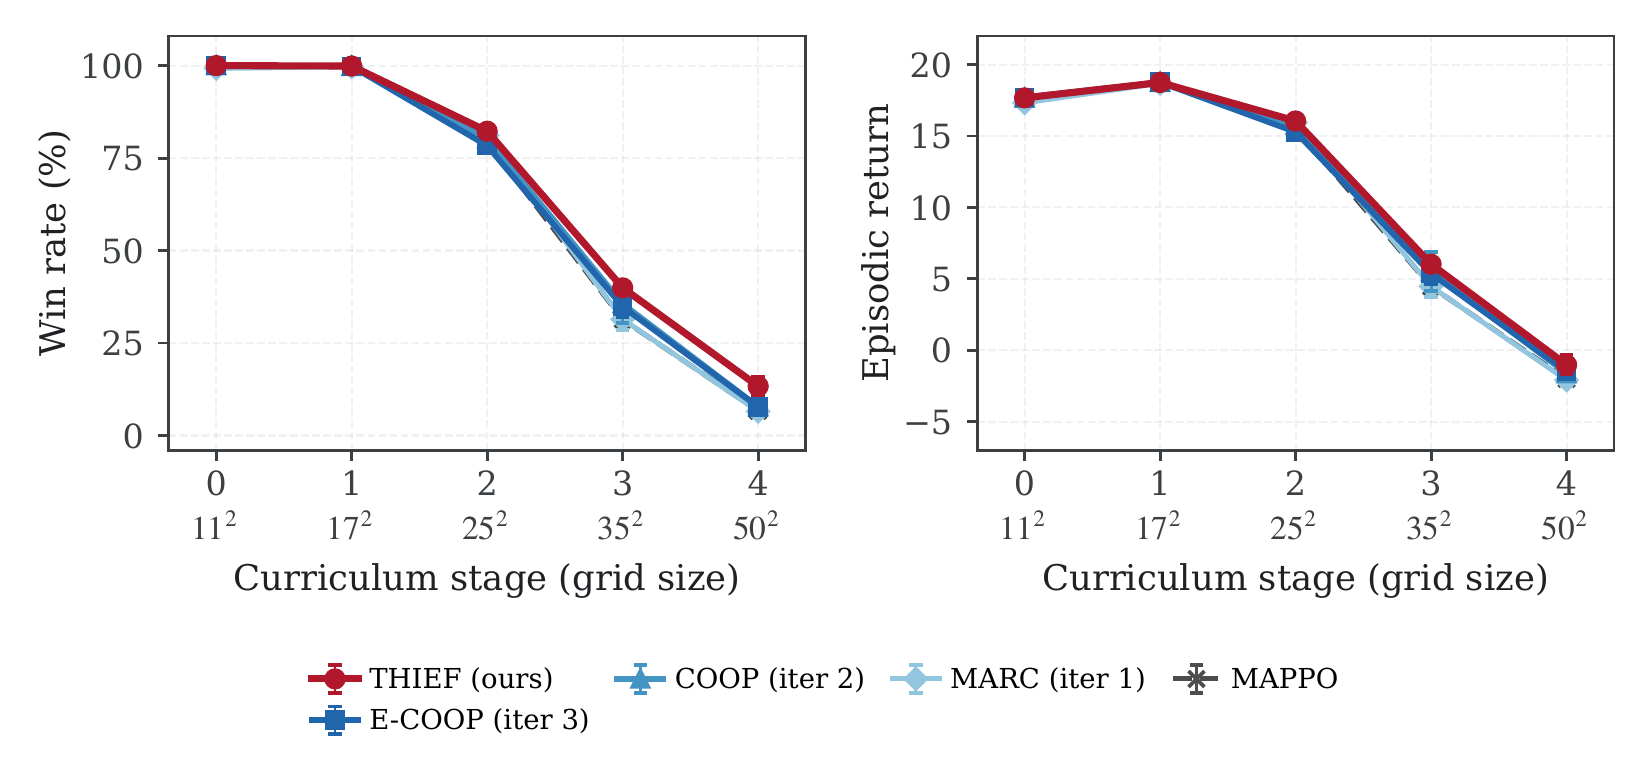
\includegraphics[width=\linewidth]{figures/curriculum_combined.pdf}
\caption{\textbf{Curriculum Scaling \& Relative Performance Advantage.} (a) Empirical win rate (\%) across HEIST curriculum Stages 1--4 ($17\times 17$ to $50\times 50$), evaluated over $N=1,\!000$ episodes per checkpoint across 10 random seeds ($10,\!000$ episodes per point, $450,\!000$ total evaluation episodes across all nine algorithms under the identical protocol). Method lineage (MARC $\to$ COOP $\to$ E-COOP $\to$ THIEF) is shown in blue shades with final THIEF in crimson; ROMA is purple, RODE is amber, and MAPPO is dark gray. Error bars denote $\pm$ one standard deviation across seeds. (b) Win rate relative advantage over the canonical MAPPO baseline ($[\text{WR}_{\text{algo}} - \text{WR}_{\text{MAPPO}}] / \text{WR}_{\text{MAPPO}} \times 100\%$). While early stages show near parity, late-stage coordination bottlenecks cause dramatic divergence: THIEF reaches a \textbf{+101.5\% relative lead} over MAPPO on Stage 4, outperforming all baselines including ROMA (+42.4\%) and COOP (+18.2\%). H-MAPPO and COMA collapse on Stages 2--4 and are omitted from curves to preserve visual resolution; their full numbers appear in Table~\ref{tab:main_results}.}
\label{fig:curriculum}
\end{figure}

\paragraph{Stage 2 (Spatial Expansion \& Multi-Patrol Evasion):}
On Stage 2 ($25 \times 25$, 2 guards, 1 camera, horizon $T_{\max}=900$), architectural divergence begins to manifest. THIEF achieves the highest performance with an \textbf{$82.2\% \pm 1.1\%$} win rate and return of $16.05 \pm 0.36$, outperforming MARC ($81.1\% \pm 1.4\%$), COOP ($80.1\% \pm 2.9\%$), MAPPO ($79.0\% \pm 2.0\%$), and ECOOP ($78.0\% \pm 1.3\%$). ROMA drops to $78.0\% \pm 1.8\%$ and RODE to $73.5\% \pm 2.1\%$---the lowest among non-hierarchical methods---as their fixed role decompositions become misaligned with the growing spatial complexity. External baselines suffer further: H-MAPPO collapses to $31.0\% \pm 5.1\%$, while COMA achieves $78.1\% \pm 3.1\%$ after prolonged exploration.

\paragraph{Stages 3 and 4 (Large-Scale Long-Horizon Coordination):}
On Stages 3 ($35 \times 35$, 3 guards, 2 cameras, 3 locked doors) and 4 ($50 \times 50$, 4 guards, 3 cameras, 4 locked doors, horizon $T_{\max}=5,\!000$), spatial and temporal horizons expand dramatically. On Stage 3, THIEF achieves a win rate of \textbf{$39.9\% \pm 1.7\%$} and return of $+6.02 \pm 0.43$, significantly outperforming COOP ($35.5\% \pm 5.3\%$), ECOOP ($34.5\% \pm 2.8\%$), MARC ($31.4\% \pm 2.9\%$), and MAPPO ($31.3\% \pm 2.6\%$). ROMA reaches $33.7\% \pm 2.1\%$ on Stage 3, between MARC and COOP with markedly lower seed variance. RODE lags at $27.2\% \pm 1.5\%$, comparable to MARC and MAPPO.

On Stage 4, the full multi-objective facility imposes extreme coordination constraints. In this long-horizon regime, most monolithic baselines degrade to $\sim 5.2\%$--$7.8\%$: MAPPO achieves $6.6\% \pm 1.4\%$, MARC reaches $6.5\% \pm 1.2\%$, E-COOP reaches $7.6\% \pm 1.4\%$, COOP reaches $7.8\% \pm 1.7\%$, and RODE achieves $5.2\% \pm 1.0\%$. Hierarchical H-MAPPO drops to $4.0\% \pm 1.1\%$, while COMA collapses to $1.4\% \pm 1.5\%$. Notably, ROMA achieves $9.4\% \pm 1.2\%$, the second-highest win rate overall and ahead of all other baselines including COOP ($7.8\%$). In contrast, THIEF achieves an authoritative win rate of \textbf{$13.3\% \pm 2.4\%$} (IQM: $13.0\%$, return: $-1.02 \pm 0.67$). This represents a \textbf{+70.5\% relative advantage} over the strongest non-ROMA baseline (COOP), a \textbf{+101.5\% advantage} over standard MAPPO, and a \textbf{+41.5\% advantage} over the strongest baseline overall (ROMA).

\paragraph{Statistical Significance (Welch's Two-Sample $t$-Tests):}
Because our benchmark comprises 10 independent training seeds, we perform two-sample Welch's $t$-tests comparing THIEF against all eight baselines on Stage 4. THIEF's advantages are statistically significant across every comparison:
\begin{itemize}[leftmargin=*,nosep]
    \item THIEF vs.\ E-COOP: $t = 6.425, \, df = 14.4, \, p = 1.4 \times 10^{-5}$
    \item THIEF vs.\ COOP: $t = 5.889, \, df = 16.0, \, p = 2.3 \times 10^{-5}$
    \item THIEF vs.\ MAPPO: $t = 7.579, \, df = 14.3, \, p = 2.2 \times 10^{-6}$
    \item THIEF vs.\ MARC: $t = 7.986, \, df = 13.0, \, p = 2.3 \times 10^{-6}$
    \item THIEF vs.\ RODE: $t = 9.700, \, df = 12.1, \, p = 4.7 \times 10^{-7}$
    \item THIEF vs.\ H-MAPPO: $t = 11.015, \, df = 12.8, \, p = 6.6 \times 10^{-8}$
    \item THIEF vs.\ COMA: $t = 13.190, \, df = 15.2, \, p = 1.0 \times 10^{-9}$
    \item THIEF vs.\ ROMA: $t = 4.514, \, df = 13.2, \, p = 5.6 \times 10^{-4}$---ROMA ($9.4\% \pm 1.2\%$) is the closest competitor and the only baseline with lower seed variance than THIEF, yet the gap remains significant at the $10^{-3}$ level.
\end{itemize}

\FloatBarrier
\subsection{Tactical Subtask Diagnostics \& Coordination Bottlenecks}
\label{sec:subtask_analysis}

To understand the mechanistic source of THIEF's performance advantage, we evaluate role-specific subtask metrics across curriculum stages (detailed in Figure~\ref{fig:subtasks} and Table~\ref{tab:subtasks_stage3}, Appendix~\ref{sec:app_subtasks}). Across all evaluated methods, early-phase subtasks are mastered robustly on Stage 3: Scout POI tagging exceeds $96\%$ for every method ($98.7\%$ or higher for all non-hierarchical methods) and Muscle guard neutralization exceeds $92.0\%$. However, the critical operational bottleneck occurs during sequential terminal override and payload extraction:

\begin{figure}[htbp]
\centering
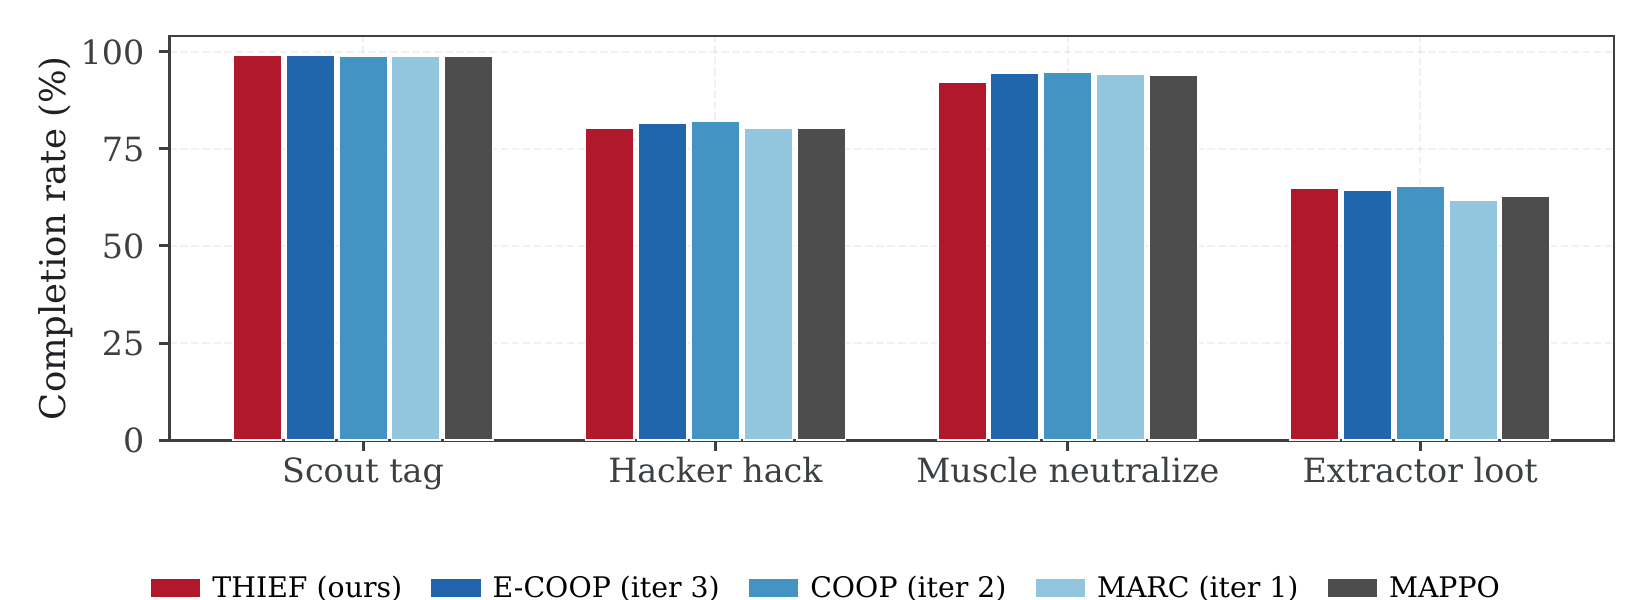
\includegraphics[width=\linewidth]{figures/stage3_subtasks.pdf}
\caption{\textbf{Role Subtask Success Rates on Stage 3.} Grouped bar breakdown of role-specific subtask completion rates for the proposed method (THIEF), key ablation (COOP), and external baselines (ROMA, MAPPO, H-MAPPO) on Stage 3 ($35\times 35$, 3 guards, 2 cameras, 3 locked doors), evaluated over $N=1,\!000$ episodes across 10 random training seeds ($10,\!000$ episodes per algorithm). While non-hierarchical methods reliably clear initial tagging and guard neutralization ($>92\%$), hierarchical H-MAPPO suffers catastrophic degradation at the terminal hacking ($40.5\%$) and payload extraction ($21.4\%$) stages, confirming that high-level goal abstraction misaligns with fine-grained spatial stealth.}
\label{fig:subtasks}
\end{figure}

\begin{itemize}[leftmargin=*,nosep]
    \item \textbf{Terminal Hacking Fidelity:} THIEF and COOP maintain over $80.3\%$--$81.9\%$ terminal hacking completion, while H-MAPPO drops to $40.5\%$ because high-level managerial sub-goals fail to account for fine-grained guard line-of-sight cones.
    \item \textbf{Extractor Vault Looting:} Vault breaching requires synchronized timing: the Hacker must disable cameras while the Muscle prevents guard interference. THIEF achieves $65.0\%$ loot acquisition on Stage 3, and safely extracts an average of $2.37$ agents per episode.
    \item \textbf{Stage 4 Failure Modes:} Trajectory analysis on Stage 4 reveals that $70.2\%$ of THIEF's unsuccessful episodes are caused by exceeding the alarm ceiling ($\alpha \ge 175$) during prolonged extraction phases, while $29.8\%$ terminate on the step horizon ($T=5,\!000$). For H-MAPPO, $45.3\%$ of failures result from step exhaustion, indicating managerial navigation paralysis.
\end{itemize}

\FloatBarrier
\subsection{Generalization to External Benchmarks: Level-Based Foraging}
\label{sec:results_lbf}

To evaluate whether the empirical advantages of deficit-targeted dynamic modularity generalize beyond the custom HEIST environment to established multi-agent benchmarks, we benchmark THIEF against ROMA~\cite{wang2020roma}, RODE~\cite{wang2021rode}, MAPPO~\cite{yu2022surprising}, H-MAPPO (our FeUdal~\cite{vezhnevets2017feudal} adaptation of MAPPO), and COMA~\cite{foerster2018counterfactual} on the canonical Level-Based Foraging (LBF) testbed~\cite{papoudakis2021benchmarking}. Table~\ref{tab:lbf_benchmark} summarizes episodic returns and cooperative food collection rates across 5 independent random seeds ($N=100$ evaluation episodes per seed, 500 episodes total per algorithm).

% Benchmark results on canonical Level-Based Foraging (LBF).
\begin{table}[htbp]
\centering
\caption{Benchmark results on the canonical Level-Based Foraging (LBF) multi-agent testbed \cite{papoudakis2021benchmarking} across two cooperative configurations (H-MAPPO is our adaptation of FeUdal Networks \cite{vezhnevets2017feudal} to MAPPO \cite{yu2022surprising}). All methods are \emph{trained} with identical PPO budgets (lr $2.5{\times}10^{-4}$, $\gamma{=}0.99$, GAE $\lambda{=}0.95$, clip $0.2$, 4 update epochs, $T{=}125$ rollout) and evaluated greedily over 5 independent seeds. Bold denotes highest performance.}
\label{tab:lbf_benchmark}
\vspace{0.04in}
\footnotesize
\setlength{\tabcolsep}{4.0pt}
\renewcommand{\arraystretch}{1.08}
\begin{tabular}{l cc cc}
\toprule
 & \multicolumn{2}{c}{\textbf{8$\times$8, 2-Player (Forced Coop)}} & \multicolumn{2}{c}{\textbf{8$\times$8, 3-Player (Asymmetric)}} \\
\cmidrule(lr){2-3} \cmidrule(lr){4-5}
\textbf{Algorithm} & \textbf{Return} & \textbf{Food (\%)} & \textbf{Return} & \textbf{Food (\%)} \\
\midrule
\textbf{THIEF (Ours)} & \textbf{0.21\scriptsize$\pm$0.04} & \textbf{26.3\%} & 0.14\scriptsize$\pm$0.03 & 21.3\% \\
ROMA \cite{wang2020roma} & 0.16\scriptsize$\pm$0.02 & 19.3\% & 0.28\scriptsize$\pm$0.28 & 32.1\% \\
RODE \cite{wang2021rode} & 0.04\scriptsize$\pm$0.01 & 4.7\% & 0.03\scriptsize$\pm$0.00 & 4.9\% \\
MAPPO \cite{yu2022surprising} & 0.14\scriptsize$\pm$0.07 & 17.8\% & 0.23\scriptsize$\pm$0.18 & 29.6\% \\
H-MAPPO \cite{vezhnevets2017feudal,yu2022surprising} & 0.20\scriptsize$\pm$0.06 & 24.5\% & \textbf{0.33\scriptsize$\pm$0.31} & \textbf{37.9\%} \\
COMA \cite{foerster2018counterfactual} & 0.04\scriptsize$\pm$0.03 & 5.4\% & 0.01\scriptsize$\pm$0.01 & 1.1\% \\
\bottomrule
\end{tabular}
\end{table}


Across both cooperative configurations, THIEF achieves strong multi-agent coordination:
\begin{itemize}[leftmargin=*,nosep]
    \item \textbf{Two-Player Coordination (\texttt{Foraging-8x8-2p-3f-v3}):} THIEF achieves the highest food collection rate (\textbf{26.3\%}) and return ($0.211 \pm 0.036$) among all methods. MAPPO ($17.8\%$) and COMA ($5.4\%$) struggle with the sparse multi-agent coordination bottleneck. H-MAPPO reaches $24.5\%$, competitive but with higher variance. ROMA achieves $19.3\% \pm 2.3\%$ and RODE $4.7\% \pm 0.9\%$---RODE's poor performance stems from its fixed binary action decomposition (locomotion vs.\ foraging roles), which collapses when food requires simultaneous cooperative loading, as the prescribed role partition does not align with the task's coordination structure.
    \item \textbf{Three-Player Coordination (\texttt{Foraging-8x8-3p-3f-v3}):} This setting introduces a three-player cooperative challenge. H-MAPPO achieves the highest raw food collection ($37.9\%$) and ROMA second ($32.1\%$), but both exhibit extremely high variance across seeds (std $30.8\%$ and $27.6\%$ respectively), indicating brittle, seed-dependent convergence rather than robust coordination. MAPPO ($29.6\%$) similarly shows high variance ($18.4\%$ std). THIEF achieves $21.3\%$ with a markedly lower standard deviation ($4.0\%$ std), demonstrating consistent coordination across seeds. RODE collapses to $4.9\%$ for the same structural reasons as the two-player task---its fixed role partition cannot adapt to the three-agent loading topology. COMA collapses to $1.1\%$ due to the combinatorial explosion of joint action spaces in the three-player setting.
\end{itemize}

\FloatBarrier
